\documentclass{sigchi}

% Use this section to set the ACM copyright statement (e.g. for
% preprints).  Consult the conference website for the camera-ready
% copyright statement.

% Copyright
\CopyrightYear{2017}
%\setcopyright{acmcopyright}
\setcopyright{acmlicensed}
%\setcopyright{rightsretained}
%\setcopyright{usgov}
%\setcopyright{usgovmixed}
%\setcopyright{cagov}
%\setcopyright{cagovmixed}
% DOI
\doi{http://dx.doi.org/10.475/123_4}
% ISBN
\isbn{123-4567-24-567/08/06}
%Conference
\conferenceinfo{HAI'17,}{October 17--20, 2016, Bielefeld, Germany}
%Price
\acmPrice{\$15.00}

% Use this command to override the default ACM copyright statement
% (e.g. for preprints).  Consult the conference website for the
% camera-ready copyright statement.

%% HOW TO OVERRIDE THE DEFAULT COPYRIGHT STRIP --
%% Please note you need to make sure the copy for your specific
%% license is used here!
% \toappear{
% Permission to make digital or hard copies of all or part of this work
% for personal or classroom use is granted without fee provided that
% copies are not made or distributed for profit or commercial advantage
% and that copies bear this notice and the full citation on the first
% page. Copyrights for components of this work owned by others than ACM
% must be honored. Abstracting with credit is permitted. To copy
% otherwise, or republish, to post on servers or to redistribute to
% lists, requires prior specific permission and/or a fee. Request
% permissions from \href{mailto:Permissions@acm.org}{Permissions@acm.org}. \\
% \emph{CHI '16},  May 07--12, 2016, San Jose, CA, USA \\
% ACM xxx-x-xxxx-xxxx-x/xx/xx\ldots \$15.00 \\
% DOI: \url{http://dx.doi.org/xx.xxxx/xxxxxxx.xxxxxxx}
% }


\toappear{
\scriptsize Permission to make digital or hard copies of all or part of this work
for personal or classroom use is granted without fee provided that
copies are not made or distributed for profit or commercial advantage
and that copies bear this notice and the full citation on the first
page. Copyrights for components of this work owned by others than ACM
must be honored. Abstracting with credit is permitted. To copy
otherwise, or republish, to post on servers or to redistribute to
lists, requires prior specific permission and/or a fee. Request
permissions from permissions@acm.org. \\
{\emph{HAI 2017, October 17--20, 2017, Bielefeld, Germany..} } \\
Copyright \copyright~2017 Association of Computing Machinery. \\
ACM ISBN 978-1-4503-5113-3/17/10\ ...\$15.00. \\
http://dx.doi.org/10.1145/XXX.XXXXX}
% Update the XXXX string to your assigned DOI from ACM.

\clubpenalty=10000
\widowpenalty = 10000



% Arabic page numbers for submission.  Remove this line to eliminate
% page numbers for the camera ready copy
% \pagenumbering{arabic}

% Load basic packages
\usepackage{balance}       % to better equalize the last page
\usepackage{graphics}      % for EPS, load graphicx instead
\usepackage[T1]{fontenc}   % for umlauts and other diaeresis
\usepackage{txfonts}
\usepackage{mathptmx}
\usepackage[pdflang={en-US},pdftex]{hyperref}
\usepackage{color}
\usepackage{booktabs}
\usepackage{textcomp}

% Some optional stuff you might like/need.
\usepackage{microtype}        % Improved Tracking and Kerning
% \usepackage[all]{hypcap}    % Fixes bug in hyperref caption linking
\usepackage{ccicons}          % Cite your images correctly!
% \usepackage[utf8]{inputenc} % for a UTF8 editor only

% If you want to use todo notes, marginpars etc. during creation of
% your draft document, you have to enable the "chi_draft" option for
% the document class. To do this, change the very first line to:
% "\documentclass[chi_draft]{sigchi}". You can then place todo notes
% by using the "\todo{...}"  command. Make sure to disable the draft
% option again before submitting your final document.
\usepackage{todonotes}

\usepackage{eurosym}

% Paper metadata (use plain text, for PDF inclusion and later
% re-using, if desired).  Use \emtpyauthor when submitting for review
% so you remain anonymous.
% \def\plaintitle{SIGCHI Conference Proceedings Format}
\def\plaintitle{Towards the Analysis of Movement Variability in Human-Humanoid
Imitation Activities}

\def\plainauthor{First Author, Second Author, Third Author,
  Fourth Author, Fifth Author, Sixth Author}
\def\emptyauthor{}
\def\plainkeywords{Authors' choice; of terms; separated; by
  semicolons; include commas, within terms only; required.}
\def\plaingeneralterms{Documentation, Standardization}

% llt: Define a global style for URLs, rather that the default one
\makeatletter
\def\url@leostyle{%
  \@ifundefined{selectfont}{
    \def\UrlFont{\sf}
  }{
    \def\UrlFont{\small\bf\ttfamily}
  }}
\makeatother
\urlstyle{leo}

% To make various LaTeX processors do the right thing with page size.
\def\pprw{8.5in}
\def\pprh{11in}
\special{papersize=\pprw,\pprh}
\setlength{\paperwidth}{\pprw}
\setlength{\paperheight}{\pprh}
\setlength{\pdfpagewidth}{\pprw}
\setlength{\pdfpageheight}{\pprh}

% Make sure hyperref comes last of your loaded packages, to give it a
% fighting chance of not being over-written, since its job is to
% redefine many LaTeX commands.
\definecolor{linkColor}{RGB}{6,125,233}
\hypersetup{%
  pdftitle={\plaintitle},
% Use \plainauthor for final version.
%  pdfauthor={\plainauthor},
  pdfauthor={\emptyauthor},
  pdfkeywords={\plainkeywords},
  pdfdisplaydoctitle=true, % For Accessibility
  bookmarksnumbered,
  pdfstartview={FitH},
  colorlinks,
  citecolor=black,
  filecolor=black,
  linkcolor=black,
  urlcolor=linkColor,
  breaklinks=true,
  hypertexnames=false
}

% create a shortcut to typeset table headings
% \newcommand\tabhead[1]{\small\textbf{#1}}

%https://tex.stackexchange.com/questions/271627/shared-author-affiliation-in-acm-sig-proc
\def\sharedaffiliation{%
\end{tabular}
\begin{tabular}{c}}

% End of preamble. Here it comes the document.
\begin{document}

\title{\plaintitle}

\numberofauthors{3}
\author{%
\alignauthor Miguel P. Xochicale\\
\email{map479@bham.ac.uk}
%
\alignauthor Chris Baber\\
\email{c.baber@bham.ac.uk}
%
\sharedaffiliation
\affaddr{Department of Electronic, Electrical and Systems Engineering}  \\
\affaddr{University of Birmingham}   \\
\affaddr{Birmingham, B15 2TT, U.K.}
}
% \numberofauthors{3}
% \author{%
%   \alignauthor{Miguel P. Xochicale\\
%     \affaddr{University of Birmingham}\\
%     \affaddr{Birmingham, UK}\\
%     \email{map479@bham.ac.uk}}\\
%   \alignauthor{Chris Baber\\
%     \affaddr{University of Birmingham}\\
%     \affaddr{Birmingham, UK}\\
%     \email{c.baber@bham.ac.uk}}\\
% }

\maketitle






\begin{abstract}
  In this paper, we present preliminary results for the analysis of movement
  variability in human-humanoid imitation activities.
  %  with the aim of the creation of better models of interaction.
  We applied the state space reconstruction's theorem which help us to have
  better understanding of the movement variability than other techniques
  in time or frequency domains.
  In our experiments, we tested our hypothesis where participants,
  even performing the same arm movement, presented slight differences in
  the way they moved. With this in mind, we asked eighteen participants to
  copy NAO's arm movements while we collected data from inertial sensors
  attached to the participants' wrists and estimated the head pose using
  the OpenFace framework.
  With the proposed metric, we found that sixteen out of eighteen participants
  imitate the robot well by moving their arms symmetrically and by keeping
  their heads static; two participants however moved their head in a synchronous way
  even when the robot's head was completely static and two different participants
  moved their arms asymetrically to the robot.
  Although the work is in its early stage, we believe that such preliminary
  results are promising for applications in rehabilitation, sport science,
  entertainment or education.
\end{abstract}



\category{I.2.9.}{Robotics}{Sensors}
\category{G.3.}{PROBABILITY AND STATISTICS}{Time series analysis}
% \category{I.5.4.}{Applications}{Signal Progessing}

% \keywords{\plainkeywords}
\keywords{Human-Robot Interaction; Human-Humanoid Imitation;
Wearable Inertial Sensors; State Space Reconstruction; Nonlinear dynamics;
Dynamics Invariants}


\section{Introduction}
Movement variability is an inherent feature within a person and between persons
movements \cite{newell1993variability}. Similarly, due to the complexity of
the human motion activities (e.g. walking, running and cycling) and the
multidimensional variables that are involved in such activities,
the use of the non-linear dynamics invariants based on the state space
reconstruction have been probed to be reliable techniques for a better insight of
movement variability \cite{Frank2010,QuintanaDuque2012,Sama2013}.
% \cite{England2007}
However, not only the methodology is important when dealing with human movement
variability but also the motion capture systems which usually are expensive,
invasive or take a long-time preparation for calibration
\cite{Baltrusaitis2016,Lemaignan2016}.
With this in mind, we have found that there is little research in the area of
human-robot interaction that is focused on the quantification of movement variability
as well as the technical challenges for both
better models of interaction and more realistic scenarios of interaction.

Therefore, the paper is divided into an intuitive explanation of the state space reconstruction;
the experiment section where reasons for measurement of arm and head pose
movement are given,
as well as the hypothesis and participant of the procedure are presented;
we then show the state spaces plots and the error bars in the results section and
finalised with our conclusions.


%% EXTRA IDEA: human movement is not noise
% Recently, Herzfeld et al. \cite{Herzfeld2014}
% conducted experiments to state that movement variability is not only noise but a
% source of movement exploration which at certain point of the exploration
% such variability is becoming a source of movement exploration.


\section{METHODS}

\subsection{State Space Reconstruction's Theorem}
The purpose of the State Space Reconstruction's Theorem is to reconstruct the
topological properties of an unknown $M-$dimensional state space $s(t)$ from a
$1-$dimensional measurement $x(t)$ in order to reconstruct an $N-$dimensional
embedding space
(Figure \ref{fig:takens_theorem}).
%%---------------------------------(FIGURE)-------------------------------------
% \begin{figure}[!htb]
\begin{figure}
\centering
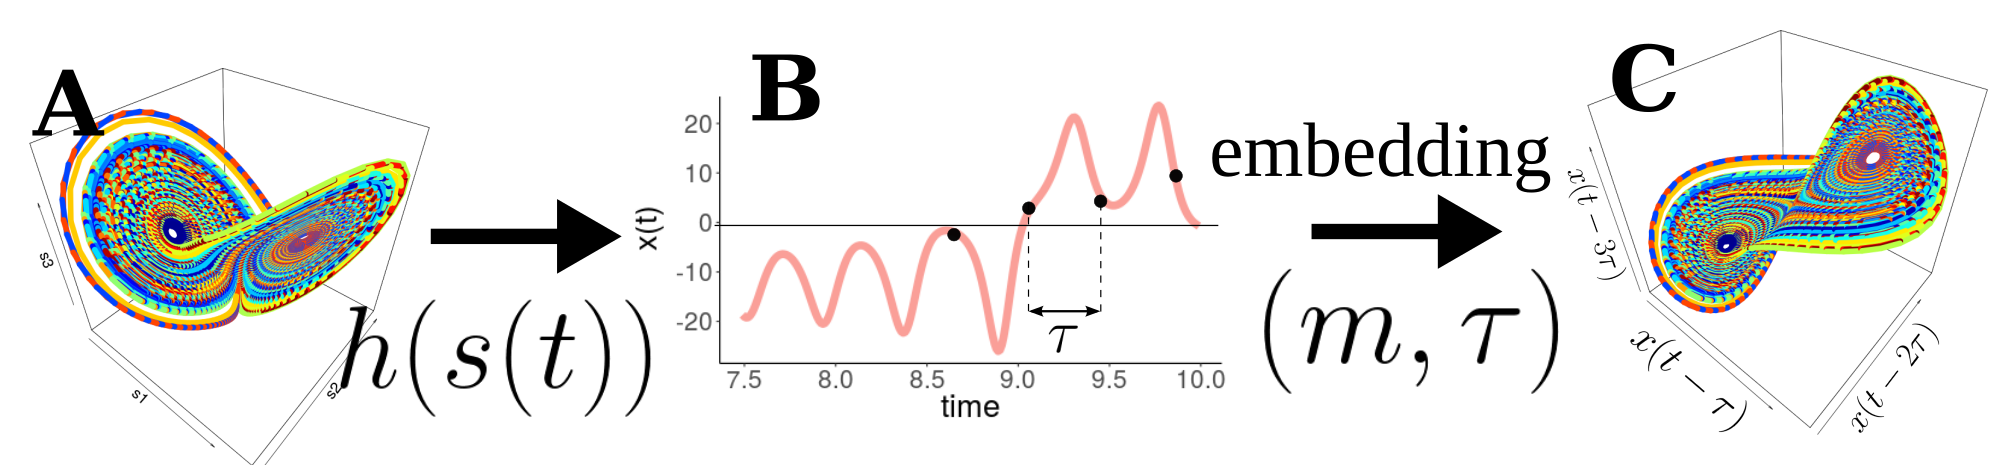
\includegraphics[width=0.45\textwidth]{figures/reconstructed_state_space/fig_v01}
\caption[PA]{State Space Reconstruction. A. $M-$dimensional state space $s(t)$;
B. $1-$dimensional measurement time-series $x(t)$; and
C. $N-$dimensional reconstructed state space $v(t)$
where $M \geq N$ (adapted from \cite{QuintanaDuque2012}).}
\label{fig:takens_theorem}
\end{figure}
%%---------------------------------(FIGURE)-------------------------------------
The time-delay embedding assumes that the time-series is a sequence $x(t)=h(s(t))$,
where $h: S \rightarrow \mathbb{R}^M$ is a measurement function on the unknown
dynamical system, being $x(t)$ observable.
Thus, the time delay reconstruction in $m$ dimensions with a time delay
$\tau$ is defined as: $\overline{x}(t) = (x(t), x(t-\tau),...,x(t-(m-1)\tau))$.
Then a further transformation is considered, e.g. PCA, in order to reduce
the dimensionality of the $m-$dimensional reconstructed state space
to a $k-$dimensional space \cite{Uzal2011}.
The advantage of the state space reconstruction's theorem is its
simplicity to reconstruct a state space where, for our case, only $1-$dimensional time-series
from either the linear acceleration of one axis the inertial sensor or the head
pose estimation from webcam can help us to have better understanding of the movement
variability. Additionally, the state space reconstruction's theorem can provide better
understanding of both correlations and symmetry of upper body movements where
techniques in time and frequency domain tent to provide little insight about the
movement variability and the structure of the time-series.

%% EXTRA IDEA
% creating assumptions for the systematic variability between persons movements.
% For this work, we assume that the
% time-series exhibit a systematic variability between persons movements.
% where $x(t)$ is produced by some time-varying system in our case the
% the persons movements.

%% EXTRA IDEA
% explore the variability between and """within""" persons movements

% EXTRA IDEA OF RELIABILITY OF METHODS
% What we do not know is how reliable the quantification methods for movement variability are
% and how the levels of imitation of a given range of movement variability can be established.

\subsection{Determining the embedding parameters ($m$ and $\tau$)}
Although State Space Reconstruction's Theorem has been used extensively in gait
recognition and walking, running and cycling activities \cite{Frank2010, QuintanaDuque2012, Sama2013},
the computation of the minimal embedding parameters largely depend on the
structure of the time-series (amplitude, frequency, nonlinearity).
To which, we however first compute the minimal embedding parameters
using the Cao's algorithm \cite{Cao1997} and the mutual information
and then we manually increase the dimensionality of the reconstructed state
space until the attractor is untangled. Refer to \cite{Cao1997}
for detailed explanation of the computation of the embedding parameters.

\section{Experiment}

\subsection{Measuring Arm Movement with Wearable Inertial Sensors}
To understand the movement variability of the participants, we use
four Wearable Inertial Sensors (SEN-10736 SparkFun 9DOF RAZOR)
which provide triple-axis accelerometer and triple-axis gyroscope (Figure~\ref{fig:exp}A).
The data were transmitted via a RN42 bluetooth module for which we set up a
sampling rate of 50 Hz and collected data using ROS \cite{quigley2009}.
The sequences ($a_x(n),a_y(n),a_z(n)$) are the raw data collected from the
triple-axis accelerometer sensor.

\subsection{Head Pose Estimation with OpenFace}
Due to the random head movements of participants while interacting with
the robot, we believe that location of the head pose can provide useful information
to have a better insight on the understanding of the movement variability.
With this in mind, we found that estimating head pose in human-robot interactions
is an active area of research where challenges like real-time tracking,
the use of less invasive equipment or the long-time preparation of calibration
techniques of the motion capture systems remain to be solved. Recently,
Lemaignan et al. \cite{Lemaignan2016}
proposed a head pose estimator using a monocular RGB webcam which is able to
track a head with rotations up to $\pm$40$^{\circ}$ horizontally and
$\pm$30$^{\circ}$ vertically.
However, OpenFace, a fully open source real-time facial behaviour analysis,
not only provides head pose (orientation and motion) but also a state-of-the-art
performance in facial landmark motion, facial expressions, and eye gaze
\cite{Baltrusaitis2016}.
For this work, we use the OpenFace because is easy to set up, is less invasive
and can provide features for facial behaviour. It can also operate with a
simple webcam in real-time (Figure~\ref{fig:exp}B).
OpenFace framework provide the location of the head with respect to camera
in millimetre (poseTx, poseTy, poseTz).


\subsection{Hypothesis}
In our previous experiments of a face-to-face human-humanoid imitation
activity \cite{Xochicale2017}, we applied the State Space Reconstruction's Theorem
to quantify the level of imitation for horizontal and vertical upper arm movements.
In such experiment, we observed in the recorded videos that effects like
boredom, fatigue or level of engagement play an important role in the influence
that each persons moves.
To which, we hypothesised, in the context of human-agent interaction
 where more realistic scenarios and better models of interaction are needed,
that not only the inertial sensors attached
to the body can provide information about movement variability but also the
facial expressions and head pose estimation.
We believe that such combination of arm movement and head pose estimation
will lead us to get better understanding of the movement variability in
human-to-humanoid activities and therefore create more reliable metrics to
quantify such movement variability.


\subsection{Participants and Procedure}
To test our hypothesis, we collected data from eighteen healthy participants:
eight male participant (age 18 $\pm$ 3.43) and ten female (age 18 $\pm$ 0.43)
in which inertial sensors were attached to the wrist of both the participant and the
humanoid robot, and put the webcam in front of the participant for the head pose
estimation (Figure~\ref{fig:exp}A).
% \subsection{Time-series from the Accelerometer Sensor}
% Then, for instance, the time-series $a_x(n)$
% with a length of $N$ samples is employed to get the embedded state space matrix,
% $\boldsymbol{E} a_{x}$, with $m$ rows and $N-(m-1)\tau$ columns.
% PCA is then applied to reduce de dimensionality of the data choosing the first
% two components of the rotated data in order to reconstruct the state space.
In the experiment, participant were asked to imitate NAO's upper arm movements
with ten repetitions (Figure~\ref{fig:nao}).
%%---------------------------------(FIGURE)-------------------------------------
% \begin{figure}[!htb]
\begin{figure}
\centering
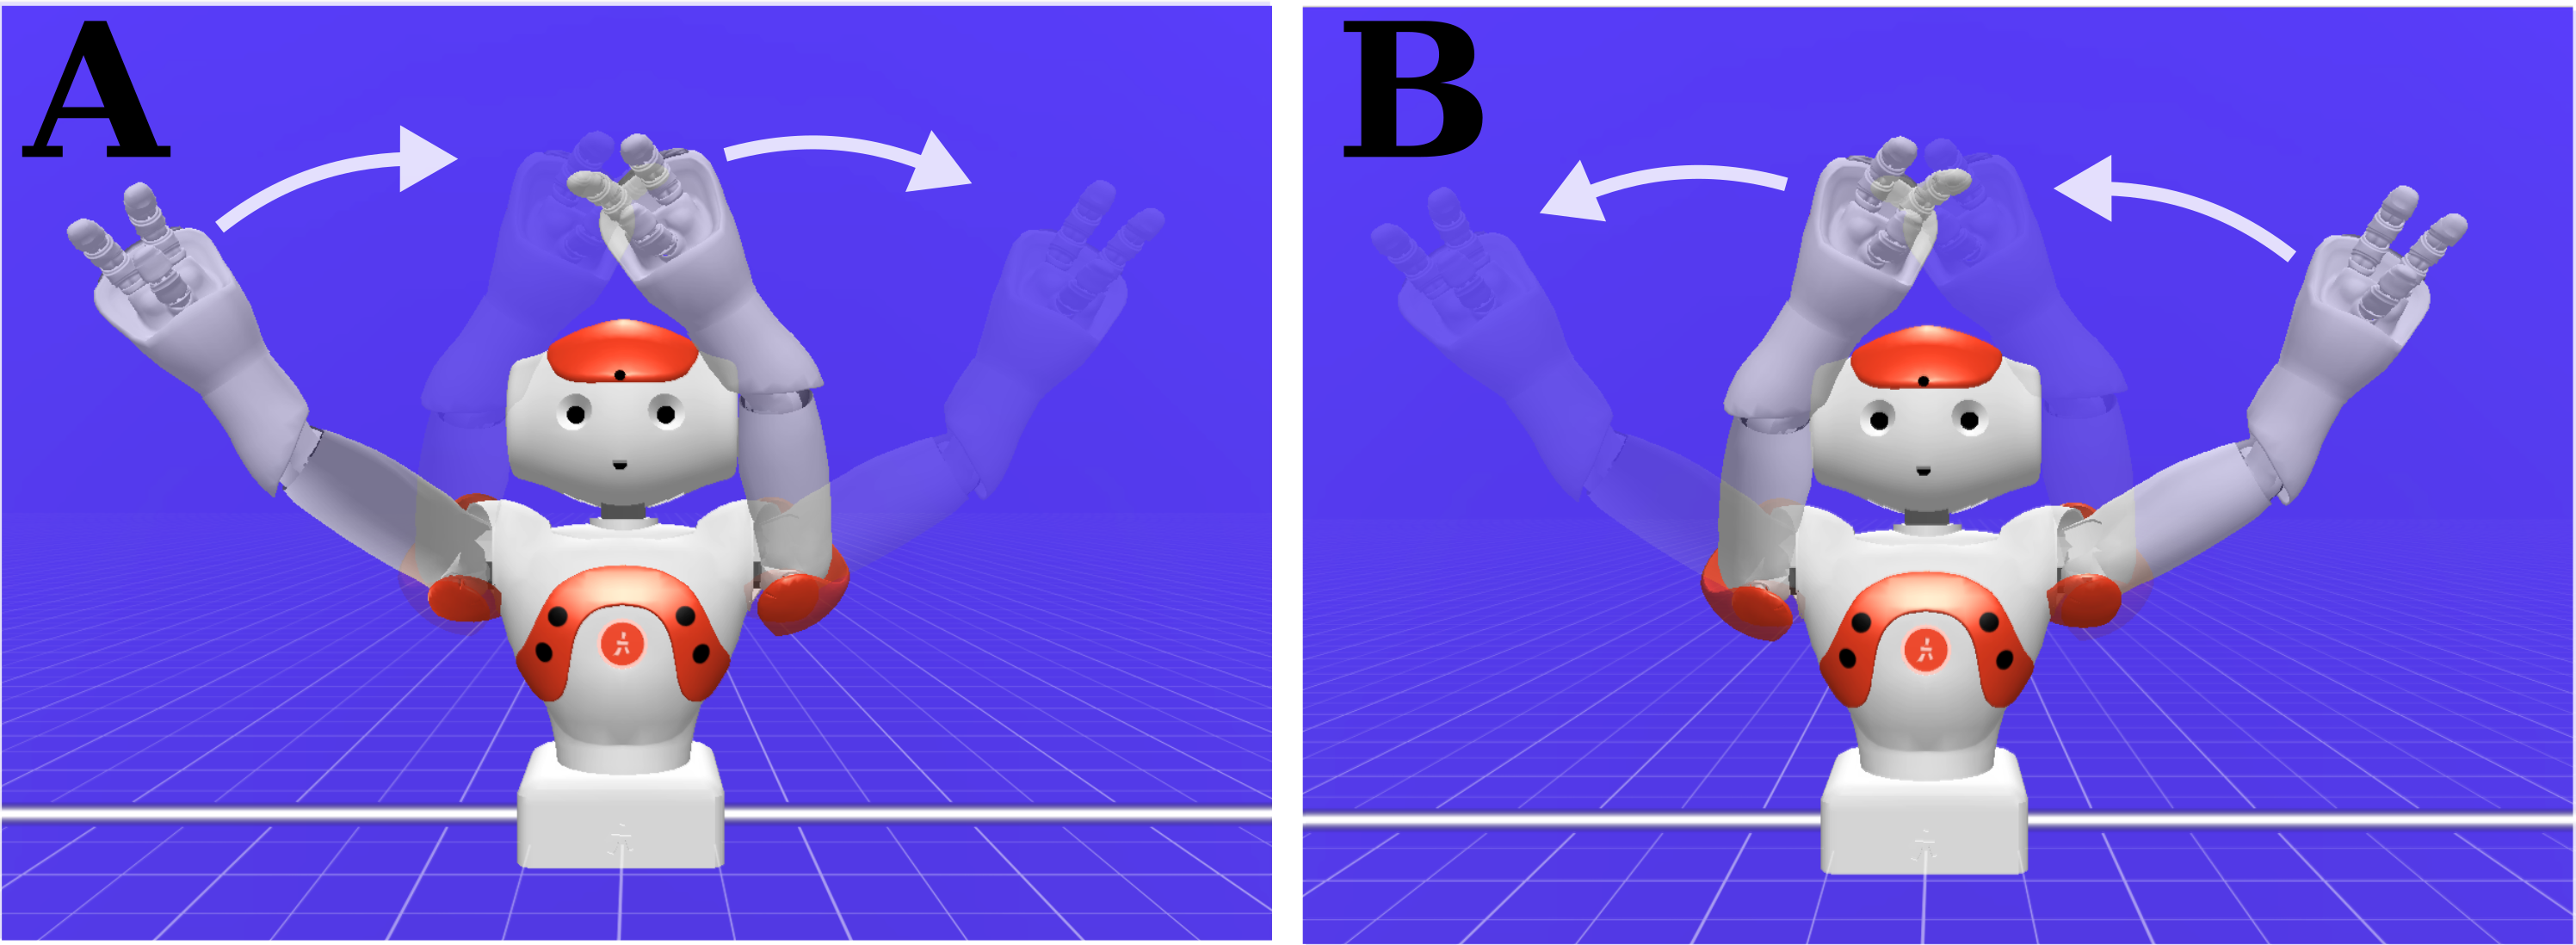
\includegraphics[width=0.45\textwidth]{figures/nao/arm_movements/fignao_v00}
\caption[PA]{NAO's arm movements: A. from right to left and B. from left to right.}
\label{fig:nao}
\end{figure}
%%---------------------------------(FIGURE)-------------------------------------
% \begin{figure}[!htb]
\begin{figure}
\centering
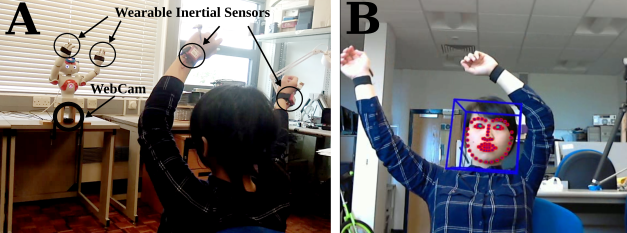
\includegraphics[width=0.45\textwidth]{figures/experiment/fig_w619h233_v2}
\caption[PA]{A. Experimental set-up of Human-Humanoid Imitation Activities;
B. Head pose estimation with OpenFace \cite{Baltrusaitis2016}.}
\label{fig:exp}
\end{figure}
%%---------------------------------(FIGURE)-------------------------------------
%%---------------------------------(FIGURE)-------------------------------------
% \begin{figure*}[!h]
\begin{figure*}[!htb]
% \begin{figure*}
\centering
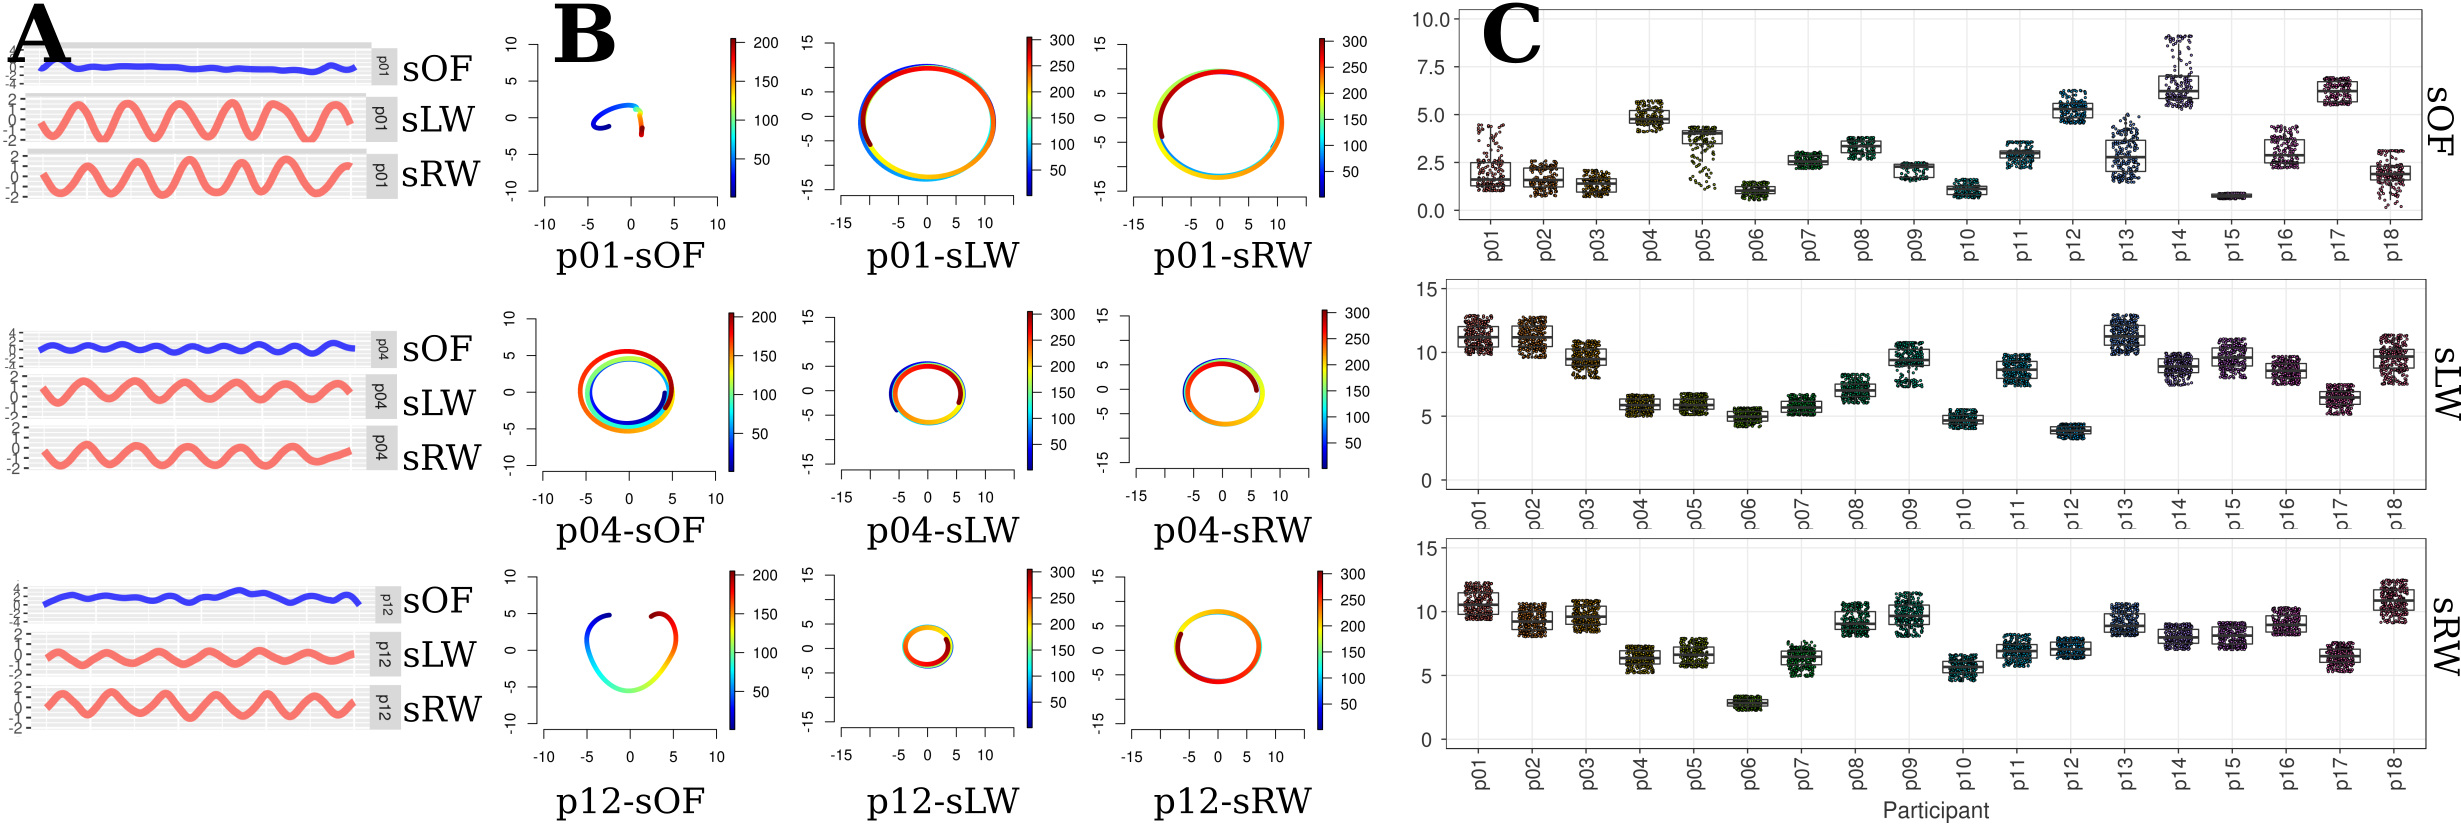
\includegraphics[width=1.00\textwidth]{figures/results/main/fig_v02}
\caption[PA]{
A. Time-series for participants p01, p04 and p12 for sensor OpenFace (sOF)
using the $x$ axis of the head pose estimation with respect to the camera,
sensor Left Wrist (sLW) and sensor Right Wrist (sRW) using the smoothed data
from the acceleremoters in x axis $a_x(n)$.
B. 2-D state space reconstruction with $m=100$ and $\tau=4$ for
participants p01, p04 and p12 using sOF, sLW and sRW.
C. Error bars for the eighteen participants for sOF, sLW and sRW. }
\label{fig:main}
\end{figure*}
%%---------------------------------(FIGURE)-------------------------------------

\section{Results}
In Figure~\ref{fig:main}, we show the time-series for the participants
p01, p04 and p12 for the $x$ axis of the head pose estimation with respect to the camera (sOF)
and the the smoothed data from the acceleremoters in x axis $a_x(n)$
for sensors attached to the Left Wrist (sLW) the Right Wrist (sRW).
We particularly observed slight similarities for the sLW and sRW time-series
for which it can be pointed out that participant p04 moved their arms symmetrically
as shown in the 2D reconstructed state space (p04-sLW and P04-sRW) and the error bars.
We also showed that participants p06 and p12 moved their arms asymmetrically as shown
in the state space reconstruction (p12-sLW and P12-sRW) and in the error bars.

With regard to the time-series from the head pose estimation sOF, we observed
that pretty much all the participants moved their heads while moving their arms.
Nonetheless, participants p04 and p17 were moving their heads in a synchronous way
with their arm movements. Such head movement of participants p04 and p17 can be
observed in the time-series p04-sOP of Figure~\ref{fig:main}A. However, the
state space reconstruction p04-sOF of Figure~\ref{fig:main}B showed a clearly
representation of such synchronicity between arm and head movements.
It can also be noticed the well distributed data in the interquartile range for
participants p04 and p17 (Figure~\ref{fig:main}C).
\section{Conclusion}
We propose the use of the state space reconstruction's theorem to analyse movement
variability in a human-humanoid imitation activity.
To which, we not only presented visual differences of movement variability
of arms and head between eighteen participants, but we also quantified such
movement variability.
For instance, sixteen out of eighteen participants imitate the robot well
by moving their arms symmetrically and by keeping their heads static, but
participants p04 and p17 moved their head in a synchronous way
even when the robot's head was completely static. We also quantified
that participants p06 and p12 did not imitate the robot well to which
their arms moved asymetrically to the robot. With this in mind, we believe
that such results are promising for applications in rehabilitation,
sport science, entertainment or education.

In future experiments, there are four areas that we intend to investigate
such as the:
(a) understanding of variability of emotions and motions in
one-to-one or one-to-many human-humanoid interactions.
(b) exploration of complex movements which can be performed by both persons and NAO;
(c) data collection from a wider range of individuals
(different gender, age and state of health) and from additional inertial sensors
attached to the body; and
(d) application of deep learning techniques to automatically classify the
movement variability.


% With the help of the state space reconstruction's theorem and with the use of
% the time-series collected through wearable inertial sensors attached to the wrist
% of participants and a webcam for head pose estimation,

%% BETTER EXPLANATION OF:
% we observed that the interquartile range of the proposed metric for participants p04 and p17
% is an indication of the movement of their heads as a tendency for the arm movements.
% With this in mind, several questions remain to be investigated

%% MORE EXPLORATION OF:
% With this in mind, we believe that such behaviour requires further investigation
% for which the motor experience affects the visual sensitivity of human action
% \cite{blake2007}.



\section{Acknowledgments}
Miguel P. Xochicale gratefully acknowledges the National Council for Science
and Technology of the United Mexican States (CONACyT) for funding his doctoral
studies at University of Birmingham, U.K.

% Balancing columns in a ref list is a bit of a pain because you
% either use a hack like flushend or balance, or manually insert
% a column break.  http://www.tex.ac.uk/cgi-bin/texfaq2html?label=balance
% multicols doesn't work because we're already in two-column mode,
% and flushend isn't awesome, so I choose balance.  See this
% for more info: http://cs.brown.edu/system/software/latex/doc/balance.pdf
%
% Note that in a perfect world balance wants to be in the first
% column of the last page.
%
% If balance doesn't work for you, you can remove that and
% hard-code a column break into the bbl file right before you
% submit:
%
% http://stackoverflow.com/questions/2149854/how-to-manually-equalize-columns-
% in-an-ieee-paper-if-using-bibtex
%
% Or, just remove \balance and give up on balancing the last page.
%
% \balance{}


% BALANCE COLUMNS
\balance{}

% REFERENCES FORMAT
% References must be the same font size as other body text.
\bibliographystyle{SIGCHI-Reference-Format}
\bibliography{references}

\end{document}

%%% Local Variables:
%%% mode: latex
%%% TeX-master: t
%%% End:
